% 原文 pp.115–121（印刷 pp.1233–1239）

% ===== 原文 p.115 =====
% 原文 §8.4（续）：Polyakov 模型的应用

不稳定性的一个可能来源是 Chern--Simons 相互作用
\begin{equation}
  \tag{8.37}
  \label{eq:8-37}
  \frac{-in}{2\pi}\int A\wedge F_A
\end{equation}
它可以加到原来的拉氏量 $\mathcal{L}$ 上。
若 $A$ 的维数为 $1/2$，则自由理论 (8.36) 是共形不变的，于是 Chern--Simons 相互作用的维数为二，因而是一个相关微扰（relevant perturbation）。
（加上 Chern--Simons 相互作用之后，拉氏量仍然是二次的。一个直接的练习——见秋季学期的作业题 FP4——表明：含该项的拉氏量描述的是一个自由的有质量理论。）

Chern--Simons 项要成为我们问题中不稳定性的来源，有两个障碍。
第一个障碍是：Chern--Simons 项中的系数 $n$ 必须是整数。
这意味着，即使你只能近似地计算这个理论，只要近似可以做得任意精确，你就能确定 $n$。
特别地，人们可以在微扰论中计算 $n$；而由于高圈项会含有 $e$ 的正幂次，它只可能来自单圈项。
因此，\emph{任何}三维规范理论中的有效 $n$ 都可以通过一次显式的单圈计算来确定。
在我们此处所考虑的具体例子中，只需注意到：Chern--Simons 项在宇称（parity）下是奇的（也就是说，它依赖于三维流形定向的选取），而我们的原理论并不如此。
宇称不变性是一圈行列式的一个对称性（无论宇称在低能下最终是否自发破缺），它保证 $n=0$。

% [Tutor Note: 这段论证靠"整性 + 解析性"两步配合，作者都写得很简。(i) 由于 $n$ 必须取整数值，它作为 $e$ 的函数不可能是连续的，故不可能是 $e$ 的非平凡函数——只能是常数；(ii) 另一方面，按 $e$ 的幂次展开时，相对 Chern--Simons 项而言 $L$ 圈（$L\ge2$）的贡献带有 $e^{2L-2}$ 的因子，在 $e\to0$ 时全部消失，于是唯一可能与 $e$ 无关的贡献来自一圈项。两步合起来即得"$n$ 等于它的单圈值"。其次，这里"维数为二"是就拉氏量\emph{密度}而言：三维中边际算符的密度维数为三，$2<3$ 故为相关算符；不要误以为 $\int A\wedge F$ 本身是某个无量纲的作用量。最后，"宇称保持 $\Rightarrow n=0$"只对纯规范理论（或宇称不变的物态）成立：若理论含手征费米子，一圈图会生成 Chern--Simons 项，$n=0$ 的结论即失效——这正是三维 Chern--Simons 物质理论中"宇称反常"的来源。]

在三维的 $U(1)$ 规范理论中，再也写不出别的相关相互作用；因此，任何能使这个理论变得不稳定的东西，都很难用 $A$ 来描述。
然而我们已看到，这个 $U(1)$ 规范理论等价（对偶）于一个标量理论
\begin{equation}
  \tag{8.38}
  \label{eq:8-38}
  \mathcal{L}=\frac{e^2}{4\pi}\int d^3x\,\partial_\alpha\phi\,\partial^\alpha\phi .
\end{equation}
在这个理论中，我们可以加上一项
\begin{equation}
  \tag{8.39}
  \label{eq:8-39}
  g\int d^3x\,\cos n\phi
\end{equation}
（对某个 $n$）。
我们之所以把势取为周期的，是因为 $\phi$ 实际上是一个到圆周的映射。
注意：$g\ne0$ 的理论有质量间隙（mass gap），而 $g=0$ 的理论没有。
于是我们指认出了某种定性地改变物理的东西，但它只能借助对偶变量才能方便地解释。
这很奇怪，因为要做对偶，本来就必须先走到低能描述中去！

这个效应在原初的 $SO(3)$ 理论中会出现吗？
我们先问：它在微扰论中会出现吗？
考虑 $SO(3)$ 理论的 Feynman 图。
我们用波浪线表示无质量模式，用实线表示有质量模式。
一个典型的 Feynman 图，例如

\begin{figure}[htbp]
  \centering
  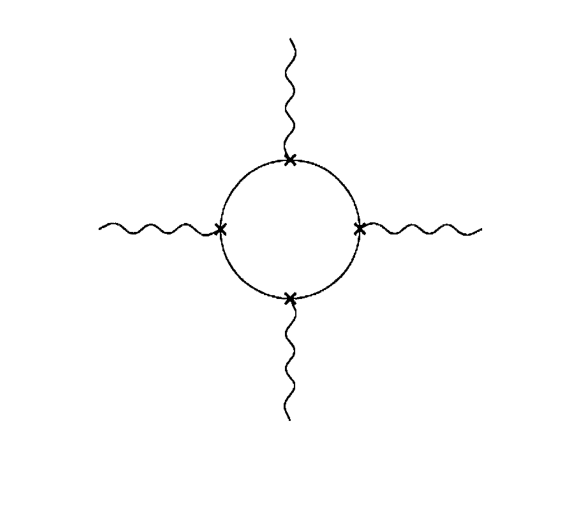
\includegraphics[width=0.34\textwidth]{figs/fig_p115_1.png}
  \caption{一个典型的单圈 Feynman 图：外线为波浪线，表示无质量模式；中间的圆圈为实线，表示有质量模式；叉号标记四个顶点。（原文图示，p.115）}
  \label{fig:p115-1}
\end{figure}

% [Tutor Note: (8.38) 的系数与后面的 (8.49)、(8.50)、(8.53)、(8.54)、(8.56) 不一致，几乎可以肯定是原文的一处笔误，正确值应为 $\frac{1}{4\pi e^{2}}$。两条独立的判据。(i) 拓扑/几何判据：三维中 Hodge $\ast$ 在二形式上是等距同构，且 $F=\ast d\phi$（作者在 p.119 明写此式），故 $F\wedge\ast F=d\phi\wedge\ast d\phi$ 逐点相等，标量理论动能项的系数必须与规范理论动能项 $\frac{1}{4\pi e^{2}}\int F\wedge\ast F$ 完全相同；而 (8.38) 印作 $\frac{e^{2}}{4\pi}$，恰好把 $e^{2}$ 从分母挪到了分子。(ii) 物理判据（更有说服力）：若动能系数为 $\kappa$，则 $\langle F F\rangle\propto\frac{1}{\kappa}\frac{1}{|x|^{3}}$，要与 (8.42) 的 $\frac{e^{2}}{|x|^{3}}$ 相符必须 $\kappa\propto\frac{1}{e^{2}}$。也就是说对偶把强弱耦合互换（$e\to1/e$），这正是三维阿贝尔对偶的标志性特征；反之，若取 (8.38) 的 $\kappa\propto e^{2}$，则 $e\ll1$（瞬子气体稀疏）时 $\phi$ 反而强耦合，p.121 上对 $\phi$ 作半经典（极小曲面）分析就完全不成立了。故 (8.38) 应读作 $\frac{1}{4\pi e^{2}}$。]

% ===== 原文 p.116 =====
这样的图将完全是温和的（tame）：我们有有质量的传播子，它们在低动量处关于动量是解析的。
这类图只是给出 $U(1)$ 规范场 $A$ 的有效作用量的修正，而这些修正可以写成拉氏量中额外的局域、规范不变的项。

\subsection{三维 $SO(3)$ 规范理论中的瞬子}
% 原文 §8.4（续）：instantons

我们需要一种完全不同的东西：\emph{瞬子}（instantons）。
让我们在 $\mathbb{R}^3$ 上工作。
我们在 $\mathbb{R}^3$ 上有一个 $SO(3)$ 丛，其结构群在无穷远处已被约化为 $U(1)$。
在无穷远处的 $S^2$ 上，一个 $U(1)$ 丛 $\mathcal{L}$ 可以有非平凡的第一 Chern 类，$c_1(\mathcal{L})\ne0$。

由于 $\mathbb{R}^3$ 是可缩的，$\mathbb{R}^3$ 上的 $SO(3)$ 丛是平凡的。
取该 $SO(3)$ 丛的一个平凡化，于是我们可以把空间 $\mathbb{R}^3$ 与丛 $\mathbb{R}^3$ 等同起来，并简单地把我们的截面 $s$ 当作一个映射 $s:\mathbb{R}^3\to\mathbb{R}^3$。
为了构造这样的、在无穷远处的 $S^2$ 上具有非平凡拓扑的映射，我们取 $s$ 形如
\begin{equation}
  \tag{8.40}
  \label{eq:8-40}
  s(\vec x)=a\,\frac{\vec x}{|x|}\,f(|x|),
\end{equation}
其中 $f(|x|)$ 是满足 $f(0)=0$、$\lim_{|x|\to\infty}f(|x|)=a$ 的递增函数，例如

\begin{figure}[htbp]
  \centering
  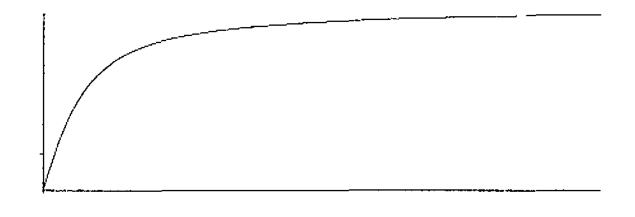
\includegraphics[width=0.52\textwidth]{figs/fig_p116_1.png}
  \caption{剖面函数 $f(|x|)$ 的图形：在原点取值为零，随 $|x|$ 单调递增，并在 $|x|\to\infty$ 时趋于常数 $a$。（原文图示，p.116）}
  \label{fig:p116-1}
\end{figure}

这样的截面在空间转动与规范转动的联合作用下不变。

我们想要这一等价类中作用量极小的解 $s$。
它应当是球对称的，渐近行为是：当 $|x|\to\infty$ 时 $Ds\sim\frac{1}{|x|^2}$。
这导致一个常微分方程，而它有唯一解。
作用量可以写成 $I/e^2$（对某个常数 $I$），因此当耦合趋于零时它发散。

注意，由于 $\vec s$ 恰好在原点处为零，结构群在原点之外被约化为 $U(1)$，但这一约化不能延拓到原点之上。
事实上，在围绕原点的球面上，该线丛具有非零的第一 Chern 类（若在 $SO(3)$ 中工作，它实际上是 $2$；也就是说，$SO(3)$ 的伴随丛在围绕原点的二维球面上分解为
\[
\mathcal{O}\oplus\mathcal{L}\oplus\mathcal{L}^{-1},
\]
其中 $\mathcal{L}$ 的次数为 $2$）。

% [Tutor Note: "次数为 $2$"是本节后面 Remark（p.120–121）的全部要害所在，作者在此只是提前使用。缘由是 $SO(3)=SU(2)/\mathbb{Z}_2$：伴随丛 $\mathcal{O}\oplus\mathcal{L}\oplus\mathcal{L}^{-1}$ 来自 $SU(2)$ 伴随丛（即三矢量表示）的分解，而在 $SU(2)$ 的语言里电荷是以 $\mathcal{L}^{1/2}$ 为基本单位的，故 $SO(3)$ 视角下的线丛是它的平方，$\deg\mathcal{L}=2\deg\mathcal{L}^{1/2}$，必为偶数；等价地说，$w_2$ 是 $c_1\bmod 2$ 的像，而 $w_2=0$ 迫使 $c_1$ 为偶。这也解释了为什么由瞬子诱导的势取 $\cos 2\phi$ 的形式（见 (8.49)、(8.54)），而不是 $\cos\phi$：写 $\cos\phi$ 会在 $\phi\to\phi+\pi$ 下变号，破坏后面要用的对称性。]

从这个观点看，一个纯粹的 $U(1)$ 理论与一个只在长距离上看起来像 $U(1)$ 的理论之间的区别在于：后者可以容许这样的丛，它们在无穷远处的大 $S^2$ 上具有非零的第一 Chern 类。
这个 Chern 类可以是我们在刚刚描述的具体解中所找到的 $2$ 的任意整数倍。

注意，在阿贝尔规范理论中，不可能使用这样的丛 $\mathcal{L}$：它在围绕原点的球面上 $c_1(\mathcal{L})\ne0$，因为这样的丛不能延拓到 $\mathbb{R}^3$ 上。
破缺到 $U(1)$ 的 $SO(3)$ 理论与 $U(1)$ 理论之间的定性差别就在于：前者允许奇点，而 $U(1)$ 描述正是在这种奇点处失效。

如果我们在 $3+1$ 维中做类似的事情，我们会得到一个能量有限（而不是作用量有限）的、与时间无关的解。
这个解看起来像坐在那里的一颗粒子，而事实上它就是一个磁单极子（magnetic monopole）。
（非零的磁荷来自 $c_1(\mathcal{L})\ne0$ 这一事实：它意味着磁场在无穷远处球面上的积分为非零值。）
作这个类比的要点在于：我们可以把瞬子设想为行为如同磁单极子的一个「零时切片」。

% ===== 原文 p.117 =====
瞬子在长距离上看起来是什么样子的？
磁单极子有一个行为如下的场
\begin{equation}
  \tag{8.41}
  \label{eq:8-41}
  F=\mathrm{const}\,\frac{\vec x}{|x|^3}=\mathrm{const}\,\frac{\hat x}{|x|^2}
\end{equation}
（由 Maxwell 方程）。

每个瞬子对路径积分的贡献是\footnote{我们用「$e$」表示规范耦合，这是阿贝尔规范理论中的标准记号。不要把它与自然对数的底「$e$」相混淆。} $e^{-I/e^2}$，当 $e$ 很小时它极其微小。

回到我们的理论，我们现在问：它在长距离上行为如何？
例如，两点函数 $\langle F(x)F(0)\rangle$ 当 $|x|\to\infty$ 时行为如何？

在自由理论中，由量纲分析，答案是 $1/|x|^3$。
（只要考虑拉氏量中的基本项 $\frac{1}{4\pi e^2}\int F\wedge\ast F$，就可以看出三维理论中曲率 $F$ 的维数为 $3/2$。）
更精确一点，我们断言
\begin{equation}
  \tag{8.42}
  \label{eq:8-42}
  \langle F_{ij}(x)F_{k\ell}(0)\rangle=\frac{e^2}{|x|^3}\left(\delta_{ik}\delta_{j\ell}+\dots\right).
\end{equation}

Feynman 图不影响这一渐近行为：$e^2$、等价地说 $1/|x|^3$ 的系数，只有很小的重整化，此外还有一些在大距离上不重要的修正。

瞬子如何影响这一分析？
考虑一个定域在 $y$ 附近的瞬子，以及它对 $x$ 与 $0$ 之间两点函数的影响。

\begin{figure}[htbp]
  \centering
  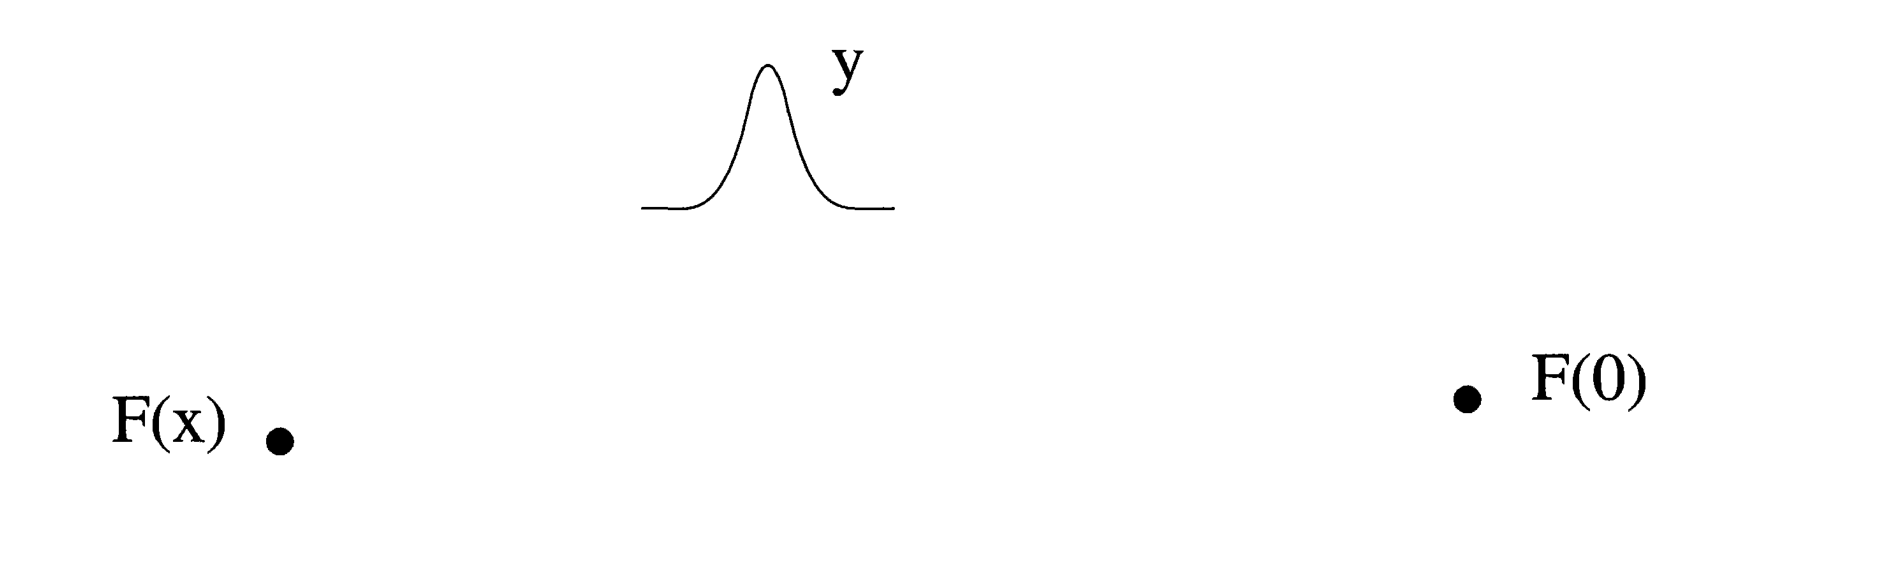
\includegraphics[width=0.66\textwidth]{figs/fig_p117_1.png}
  \caption{定域在 $y$ 附近的瞬子对两点函数 $\langle F(x)F(0)\rangle$ 的贡献示意：钟形曲线表示瞬子场强的空间分布（其峰在 $y$ 处），下方两个黑点分别标记算符插入点 $x$ 与 $0$。（原文图示，p.117）}
  \label{fig:p117-1}
\end{figure}

瞬子扇区中路径积分的首项近似是
\begin{equation}
  \tag{8.43}
  \label{eq:8-43}
  e^{-I/e^2}\int d^3y\,\frac{(\vec x-\vec y)}{|x-y|^3}\,\frac{\vec y}{|y|^3}.
\end{equation}

这里我们对瞬子的位置 $y$ 积分；被积函数就是 $F(x)F(0)$ 在瞬子场中的经典值。
我们把瞬子的经典作用量记作 $I/e^2$，并在对瞬子位置的积分中带上因子 $\exp(-I/e^2)$，因为这是存在一个瞬子的单位体积概率。
（当 $e\to0$ 时 $I$ 与 $e$ 无关。）
该积分按 $1/|x|$ 标度。
因此，把微扰贡献与瞬子修正相加，总的行为是
\begin{equation}
  \tag{8.44}
  \label{eq:8-44}
  \langle F(\vec x)F(\vec 0)\rangle\cong\frac{1}{Z}\Bigl(\text{pert. theory}+e^{-I/e^2}(\text{instanton sector})\Bigr)
\end{equation}
\begin{equation}
  \tag{8.45}
  \label{eq:8-45}
  \cong\frac{1}{Z}\left((1+\dots)\frac{1}{|x|^3}+e^{-I/e^2}\Bigl(\frac{1}{|x|}+\dots\Bigr)\right).
\end{equation}

% [Tutor Note: 作者说 (8.43) "按 $1/|x|$ 标度"，这一步跳过了一个容易忽略的细节：$\int d^3y\,\frac{1}{|x-y|^3}\frac{1}{|y|^3}$ 在 $y\to0$ 处是\emph{对数发散}的（$\frac{d^3y}{|y|^3}\sim\frac{dy}{y}$），在 $y\to\infty$ 处则收敛。故所谓 $1/|x|$ 只是首项标度，真实的积分还要乘一个 $\ln(\text{瞬子尺度}/|x|)$ 型的对数因子，截断尺度由瞬子的大小（即经典解的芯）给出。这也提醒：把瞬子当作点荷来处理，在 $y$ 靠近 $x$ 或 $0$ 时是不成立的，(8.43) 的被积函数在这些区域本应换成瞬子解的真实场强。]

% ===== 原文 p.118 =====
由于瞬子贡献在红外比自由理论项更重要（$1/|x|$ 对 $1/|x|^3$），瞬子引发了一个不稳定性。

为了更细致地看清红外到底发生了什么，我们首先注意到：瞬子是\emph{稀少}的。
在小体积 $V_0$ 中存在一个瞬子的概率正比于 $V_0e^{-I/e^2}$，故每个瞬子所对应的空间体积为 $V\sim e^{I/e^2}$，而两个瞬子之间的空间间距为
\[
R\sim V^{1/3}\sim e^{I/3e^2}.
\]

然而在红外，如果我们考虑足够大的空间体积，就会得到大量的瞬子，可以把它们当作由确定大小的粒子组成的气体。
这些粒子是\emph{带电}的，所以我们不能忽略它们之间由 Coulomb 势给出的相互作用。
图像如下：

\begin{figure}[htbp]
  \centering
  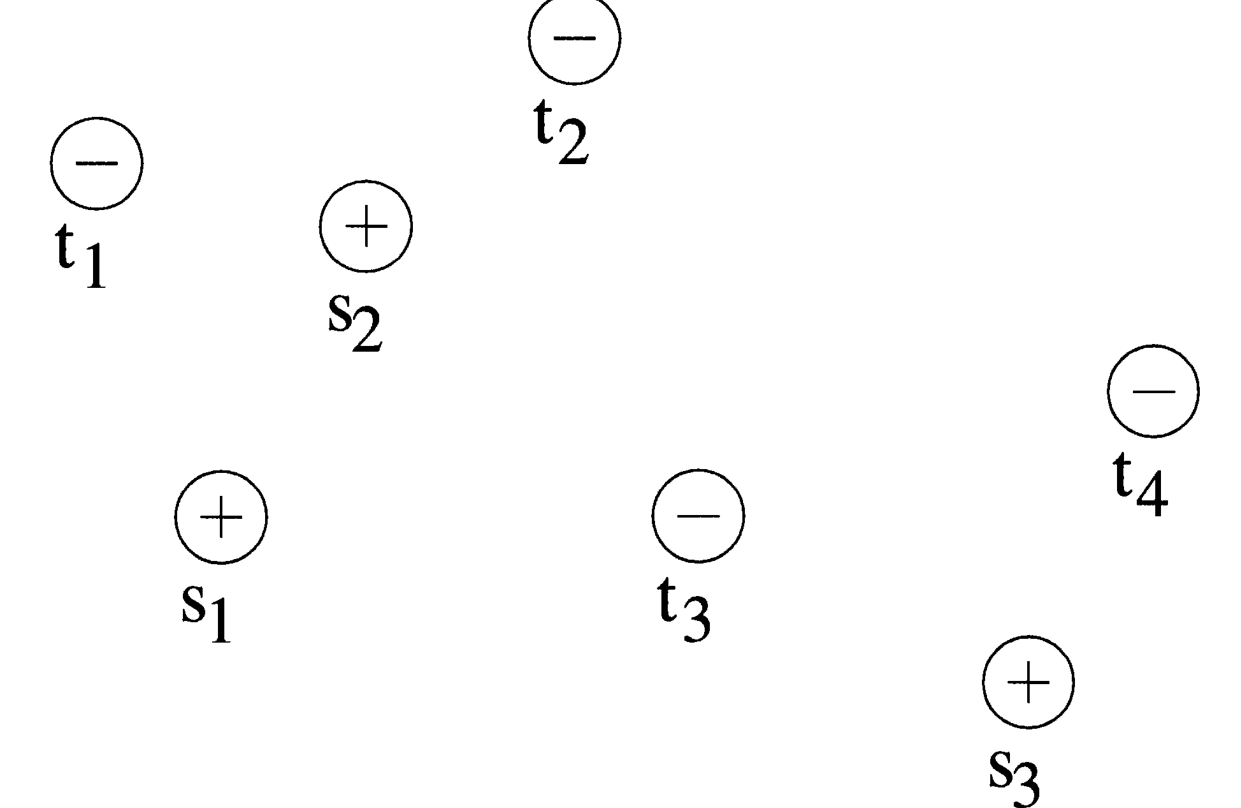
\includegraphics[width=0.52\textwidth]{figs/fig_p118_1.png}
  \caption{三维空间中的瞬子气体：标有 $+$ 的圆圈表示带正荷的瞬子，位置记为 $s_i$；标有 $-$ 的圆圈表示带负荷的反瞬子，位置记为 $t_j$。（原文图示，p.118）}
  \label{fig:p118-1}
\end{figure}

我们用 $s_i$ 标记瞬子（带正荷）的位置，用 $t_j$ 标记反瞬子（带负荷）的位置。
对所有这些求和得到
\begin{align}
  \sum_{n,m=0}^{\infty}\frac{1}{n!m!}&\int d^3s_i\big|_{i=1}^{n}\int d^3t_j\big|_{j=1}^{m}\exp\left(-\frac{I}{e^2}(n+m)\right)\notag\\
  \tag{8.46}
  \label{eq:8-46}
  &\times\exp\left(\frac{1}{4\pi e^2}\sum_{i<j}\left(\frac{1}{|s_i-s_j|}+\frac{1}{|t_i-t_j|}\right)-\frac{1}{4\pi e^2}\sum_{i,j}\frac{1}{|s_i-t_j|}\right).
\end{align}

在被积函数中，我们写出了一个位形的作用量的指数，该位形由位于点 $s_i$ 的彼此远离的瞬子与位于点 $t_j$ 的反瞬子组成。
作用量中的主要项就是 $(n+m)I$，如同瞬子与反瞬子之间没有相互作用。
但此外还有一个相互作用势
\begin{equation}
  \tag{8.47}
  \label{eq:8-47}
  \frac{1}{4\pi e^2}\,\frac{1}{|s_i-s_j|}
\end{equation}
作用在位于 $s_i$、$s_j$ 的瞬子之间；对两个反瞬子或一个瞬子与一个反瞬子，有类似的项，分别正比于 $1/|t_i-t_j|$ 或 $-1/|s_i-t_j|$。
这些项合起来就是瞬子之间的经典「Coulomb 势」。
在三维中瞬子表现得像「带磁荷的粒子」；三维中相距 $r$ 的两个带电粒子之间的相互作用势正比于 $1/r$，这就给出了所说的那些相互作用项。
瞬子之间存在的这些长程相互作用，正是当前问题与我们上周在一个更初等的例子中研究过的稀疏瞬子气体之间的区别。

% [Tutor Note: (8.46) 的相互作用项符号与 (8.53) 相反，二者必有一处笔误，而几乎可以断定是 (8.46)。理由有二。(i) 两式写的是同一个量：(8.53) 正是对 (8.52)（即 (8.46) 的场论改写）作高斯积分的结果，作者自己也说 "We thus recover the previous formula"；把两式对照可见，同号对（$s$--$s$、$t$--$t$）前面的符号恰好相反。(ii) 物理上瞬子带同号磁荷、彼此排斥，相距 $r$ 时二者的作用量为 $+\frac{1}{4\pi e^{2}r}$，故权重 $e^{-S}$ 中同号对应\emph{负}号、异号（瞬子—反瞬子）对应\emph{正}号——这正是 (8.53) 的写法；若照 (8.46) 印出的符号，同号瞬子将相互\emph{吸引}、异号将相互\emph{排斥}，就不成其为等离子体，下面赖以产生质量间隙的 Debye 屏蔽（需要异号聚集、同号排开）也无从谈起。因此 (8.46) 的第二个 $\exp$ 应整体再添一个负号。附带一提：同号对用 $\sum_{i<j}$（每个无序对只数一次）、异号对用完整的 $\sum_{i,j}$（每对只涉及一个 $s$ 与一个 $t$，本无重复计数），这两处指标写法的差别不是笔误，不能统一成同一种求和。]

% ===== 原文 p.119 =====
\subsection{瞬子气体与 Debye 屏蔽}

为了计算所需的 $F$ 的两点函数，我们还需要一个算符插入，即
\begin{equation}
  \tag{8.48}
  \label{eq:8-48}
  F(x)=\sum\frac{x-s_i}{|x-s_i|^3}-\sum\frac{x-t_j}{|x-t_j|^3},
\end{equation}
（这里我们用瞬子气体中的值来近似 $F(x)$），对 $F(0)$ 也类似。

执行求和 (8.46) 所涉及的物理，是空间中一等离子体（plasma）的经典统计力学：其化学势为 $I/e^2$，能量 $E$ 由瞬子与反瞬子之间的 Coulomb 势给出，温度为 $T=4\pi e^2$。

我们需要的现象称为「Debye 屏蔽」（Debye screening）——等离子体会屏蔽外电荷。
由于这种屏蔽，系统将具有质量间隙。

下面是 Debye 屏蔽（在此语境下）的一个简短的数学推导。
我们回到低能理论，用对偶变量把它写成一个标量理论，其中 $F=\ast d\phi$。
我们将在拉氏量中加一项来计入瞬子效应；我们将要使用的项（其正当性由后面计算的结果保证）是
\[
\int e^{-I/e^2}\left(e^{2i\phi}+e^{-2i\phi}\right).
\]
（指数中出现 $2$ 是因为基本瞬子的第一 Chern 类为 $2$。）
$F$ 的算符插入于是变成 $\ast d\phi$ 的插入，而两点函数 $\langle F(x)F(0)\rangle$ 可以写成：
\begin{equation}
  \tag{8.49}
  \label{eq:8-49}
  \Omega=\int\mathcal{D}\phi\,(\ast d\phi(x))(\ast d\phi(0))\exp\left[-4\pi e^2\int|d\phi|^2+\int e^{-I/e^2}\left(e^{2i\phi}+e^{-2i\phi}\right)\right].
\end{equation}

首先我们要说明这确实是对偶变量中的正确描述，然后再分析这个表达式。

我们将把 $\Omega$ 按微扰论展开：
\begin{align}
  \Omega=\sum_{n,m=0}^{\infty}&\frac{1}{n!m!}\int\mathcal{D}\phi\,\exp\left(-\frac{1}{4\pi e^2}\int d\phi\wedge\ast d\phi\right)(\ast d\phi(x))(\ast d\phi(0))\cdot\notag\\
  \tag{8.50}
  \label{eq:8-50}
  &\cdot\left(\int e^{-I/e^2}e^{2i\phi(y)}d^3y\right)^{n}\left(\int e^{-I/e^2}e^{-2i\phi(z)}d^3z\right)^{n}.
\end{align}

我们再用下面这条原理作进一步展开：
\begin{equation}
  \tag{8.51}
  \label{eq:8-51}
  \left(\int dy\,f(y)\right)^{n}=\int dy_1\dots dy_n\,f(y_1)\dots f(y_n).
\end{equation}

于是，我们可以把 (8.50) 改写为
\begin{align}
  \Omega=\sum_{n,m=0}&\int\mathcal{D}\phi\int d^3s_i\big|_{i=1}^{n}d^3t_j\big|_{j=1}^{m}\,(\ast d\phi(x))(\ast d\phi(0))\cdot\notag\\
  \tag{8.52}
  \label{eq:8-52}
  &\cdot\exp\left(-\frac{I}{e^2}(n+m)+2i\sum_i\left(\phi(s_i)-\phi(t_i)\right)\right)\exp\left(-4\pi e^2\int|d\phi|^2\right).
\end{align}

% [Tutor Note: (8.49) 与 (8.52) 中的动能项系数印作 $-4\pi e^{2}$，与 (8.50) 的 $-\frac{1}{4\pi e^{2}}$ 以及 (8.53)、(8.54)、(8.56) 的 $\frac{1}{4\pi e^{2}}$ 明显矛盾，应是排版时把 $\frac{1}{4\pi e^{2}}$ 的分数线丢掉了（原稿很可能是 $-\frac{1}{4\pi e^{2}}\int|d\phi|^{2}$）。这里无需任何计算即可判定：$|d\phi|^{2}d^{3}x$ 与 $d\phi\wedge\ast d\phi$ 是同一个三形式，所以 (8.52) 末尾的因子 $\exp(-4\pi e^{2}\int|d\phi|^{2})$ 必须逐字等于 (8.50) 中的 $\exp(-\frac{1}{4\pi e^{2}}\int d\phi\wedge\ast d\phi)$；而 (8.52) 本来就是 (8.50) 的改写，同一个量不可能有两种系数。既然 (8.50)、(8.53)、(8.54)、(8.56) 四处一致为 $\frac{1}{4\pi e^{2}}$，出错的是 (8.49) 与 (8.52)。读者若照印出的 $4\pi e^{2}$ 去算，完成配方后得到的库仑势前因子将与 (8.46)、(8.53) 不符，屏蔽长度会带上错误的 $e$ 幂次，Debye 屏蔽的整个推导随之失效。]

% [Tutor Note: (8.50) 末尾两个因子都印成 $n$ 次幂，第二个应为 $m$ 次幂，这是原文的一处笔误。三条独立证据：(i) 前面的求和权重是 $\frac{1}{n!m!}$，若两个因子都是 $n$ 次幂，则 $m$ 只出现在 $1/m!$ 中而无任何 $m$ 依赖的积分，级数对 $m$ 求和会给出一个无意义的 $\sum_m 1/m!=e$ 因子；(ii) (8.46) 中反瞬子的个数明确是 $m$（积分 $\int d^3t_j\big|_{j=1}^{m}$）；(iii) (8.52) 把 (8.50) 的两个因子化成了 $\int d^3s_i\big|^{n}_{i=1}$ 与 $\int d^3t_j\big|^{m}_{j=1}$，说明原作者本意正是 $n$ 与 $m$。此处忠实照印，但读者应按 $m$ 理解。]

% ===== 原文 p.120 =====
完成配方后，$\phi$ 积分是高斯型的；该积分将给出一个因子
\begin{equation}
  \tag{8.53}
  \label{eq:8-53}
  \exp\left(-\frac{1}{4\pi e^2}\left(\sum_{i<j}G(s_i,s_j)+\sum_{i<j}G(t_i,t_j)-\sum_i\sum_j G(s_i,t_j)\right)\right)
\end{equation}
乘到总答案上，其中 $G(s,t)=1/|s-t|$ 是 Laplacian 的 Green 函数。
于是我们重新得到了先前的公式。

注意，我们在指数中略去了 $G(s_i,s_i)$ 与 $G(t_j,t_j)$ 这两类项。
从标量场论的观点看，略去这些项就是重整化的过程。
从原初 $SO(3)$ 规范理论的观点看，所有涉及 Green 函数的项都是在近似一个由彼此远离的瞬子与反瞬子组成的气体的作用量时出现的。
在这个处理中，对角项不会出现，因为单个瞬子（或反瞬子）的作用量已经在常数 $I/e^2$ 中计算过了，不会再出现一个发散的修正 $G(s_i,s_i)$ 或 $G(t_j,t_j)$。
因此，低能理论需要一次看似任意的重整化，而它的理由从高能理论的观点看是清楚的；这当然是一种典型的情形。

% [Tutor Note: 严格说 $G(s,t)=1/|s-t|$ 并不是按 $-\Delta G=\delta^{(3)}$ 归一化的 Green 函数，而是其 $4\pi$ 倍：$-\Delta\frac{1}{|s-t|}=4\pi\delta^{(3)}(s-t)$。作者把它称为「Laplacian 的 Green 函数」是一种约定（省略 $4\pi$），而这个 $4\pi$ 恰好被 (8.53) 外面的 $\frac{1}{4\pi e^2}$ 吸收，使指数中的库仑势正好是 (8.46) 的 $\frac{1}{4\pi e^{2}}\frac{1}{|s_i-s_j|}$。若按教科书的 $G=\frac{1}{4\pi|s-t|}$ 代入 (8.53)，就会把库仑势错误地缩小 $4\pi$ 倍。另注意 (8.53) 与 (8.46) 的差别只在相互作用项的整体符号（见上面关于 (8.46) 的批注）：(8.53) 中同号对为负、异号对为正，这在 $e^{-S}$ 的约定下正是"同号排斥、异号吸引"，也正是完成配方后各向同性高斯积分所必然给出的结构；因此可以把 (8.53) 当作判定 (8.46) 符号的独立依据。]

我们学到的教训是这样的：我们的原问题（$SO(3)$ 规范理论）在红外可以用对偶变量、借助拉氏量
\begin{equation}
  \tag{8.54}
  \label{eq:8-54}
  \frac{1}{4\pi e^2}\int|d\phi|^2+2e^{-I/e^2}\int d^3x\,\cos 2\phi
\end{equation}
来描述。
第二项是不可重整的，但它在红外行为良好。
把势在其极小值附近展开，我们看到 $\phi$ 获得了质量。
于是，原先无质量的 $U(1)$ 光子 (i) 被对偶化并重新解释为一个标量，(ii) 获得了一个在该语言中更容易描述的质量。

关于上述推导，还有另一种理解方式。
从无质量标量场出发，按本讲第 3 节的办法把它对偶化为无质量规范场 $A$。
现在给无质量标量的理论加上一个弱微扰
\[
\epsilon\int d^3x\left(e^{2i\phi}+e^{-2i\phi}\right).
\]
用规范场来表达，算符 $e^{2i\phi(P)}$ 就变成——正如我们在第 3 节末尾所指出的——一条指令：「删去点 $P$，并考虑在围绕 $P$ 的小球面上具有第一 Chern 类 $2$ 的丛。」
换句话说，从低能下看起来像 $U(1)$ 的 $SO(3)$ 理论的观点看，这条指令就是「在 $P$ 处包含一个瞬子」。
如果我们取相互作用项 $\epsilon\int d^3x\left(e^{2i\phi}+e^{-2i\phi}\right)$ 并按 $\epsilon$ 的幂次展开，我们就直接生成了瞬子气体，其中每一次 $e^{2i\phi}$ 或 $e^{-2i\phi}$ 的插入分别对应一个瞬子或反瞬子。

\subsection{禁闭}

现在我们要研究禁闭（confinement）。
一个重要的预备步骤是注意问题的对称性。
一般地，在从阿贝尔规范理论出发的对偶中，$\phi$ 是一个角变量，即到圆周的映射，所以 $\phi$ 与 $\phi+2\pi$ 等价。
然而，由于瞬子诱导的相互作用是 $2\phi$ 的三角函数，理论具有 $\phi\to\phi+\pi$ 的对称性。

\textbf{注（Remark）.}
瞬子相互作用是 $2\phi$ 的函数，因为瞬子有 $c_1=2$。
而这又是因为 $SO(3)$ 有非平凡的基本群 $\mathbb{Z}_2$，从而有非平凡的二重覆盖 $SU(2)$。
这些事实之间的联系如下。
我们的理论可以用处于 $SU(2)$ 的二维表示中的粒子来探测。
我们把无穷远处的 $SO(3)$ 丛写作 $\mathcal{O}\oplus\mathcal{L}\oplus\mathcal{L}^{-1}$。
与之相伴的 $SU(2)$ 丛（它存在，因为 $\mathbb{R}^3$ 可缩，故该 $SO(3)$

% ===== 原文 p.121 =====
丛有 $w_2=0$）则是 $\mathcal{L}^{1/2}\oplus\mathcal{L}^{-1/2}$。
线丛 $\mathcal{L}^{1/2}$ 的存在，正是 $c_1(\mathcal{L})$ 为偶数的拓扑理由，从而也是 $\phi$ 的理论具有 $\phi\to\phi+\pi$ 对称性的理由。
现在，按照第 7 讲 §8 中第一个 Remark 的说法，这个理论中禁闭的精确判据之所以存在，只是因为有可能用处于 $SU(2)$ 二维表示中的电荷（或等价地，用在中心元作用下非平凡的任意表示）来探测它。
既然这种可能性直接导致低能理论的 $\phi\to\phi+\pi$ 对称性，那么正如我们很快会看到的，这一对称性在禁闭的分析中起作用，也就是顺理成章的了。

在这个理论原来的规范理论描述中，我们可以考虑一条曲线 $C\subset M$——由于我们在三维中，它可以是一个纽结，就像图中那样！

\begin{figure}[htbp]
  \centering
  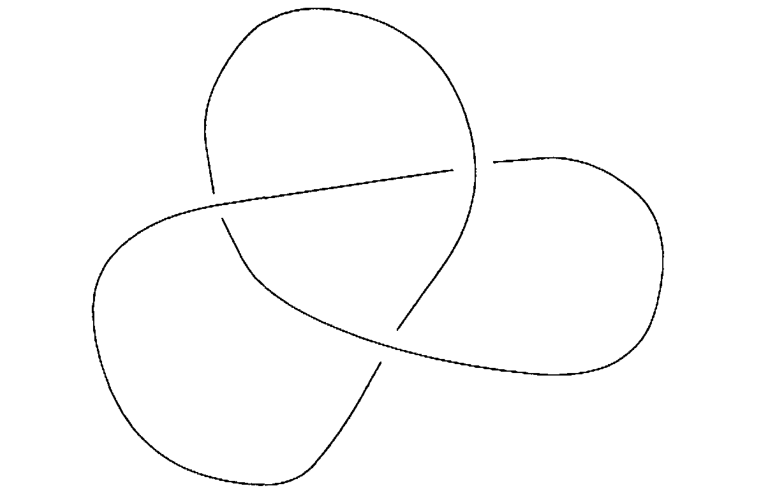
\includegraphics[width=0.44\textwidth]{figs/fig_p121_1.png}
  \caption{三维时空中的一条打结的曲线 $C\subset M$：三维空间中 Wilson 线可以打结，这是三维特有的现象。（原文图示，p.121）}
  \label{fig:p121-1}
\end{figure}

打结的 Wilson 线是我们在三维之外所没有的东西！
对给定的 $C$，我们可以考虑相应的 Wilson 线算符
\begin{equation}
  \tag{8.55}
  \label{eq:8-55}
  \left\langle\mathrm{Tr}_R\,\mathrm{Hol}(A,C)\right\rangle
\end{equation}
其中 $R$ 是 $SU(2)$ 的二维表示，$\mathrm{Hol}$ 表示和乐（holonomy）。
在我们的红外描述（用 $\phi$ 表达）中，这个算符翻译成什么？
正如我们在第 3 节末尾所看到的，它翻译成一条处方：「从时空中删去 $C$，并把 $\phi$ 解释为一个平坦圆周丛的截面，该丛的联络在绕 $C$ 一周时有单值性（monodromy）。」
单值性由角 $2\pi\lambda$ 给出，其中 $\lambda$ 是第 3 节讨论中引入的、出现在 Wilson 圈里的 $U(1)$ 荷（模 $1$）。
我们选取的是处于 $SU(2)$ 二维表示中的 Wilson 线；以 $SO(3)$ 的权格为单位，其 $U(1)$ 荷为 $\pm1/2$（这一事实在上面 Remark 中以另一种方式被利用了）。
因此我们的例子有 $\lambda=1/2$。
于是绕该圆周的单值性是 $\phi\to\phi+\pi$；正如我们刚才注意到的，即使加上了瞬子诱导的相互作用，这也是理论的一个对称性。

现在问题是经典的了：我们要找作用量
\begin{equation}
  \tag{8.56}
  \label{eq:8-56}
  \frac{1}{4\pi e^2}\int|d\phi|^2-2e^{-I/e^2}\int d^3x\left(\cos 2\phi-1\right)
\end{equation}
的极小值，其中 $\phi$ 是一个圆周取值函数，并要求它在绕 $C$ 一周时有单值性 $\pi$。
（我们平移了 $\phi$，使极小能量位于 $\phi=0,\pi$ 处；又从作用量中减去一个常数，使真空能量为零。）
于是，特别地，由于单值性的要求，$\phi$ 不能是常数。
事实上，最小作用量的解近似地由一张以 $\partial\Sigma=C$ 为边界的极小面积曲面 $\Sigma$ 给出；$\phi$ 在远离 $\Sigma$ 处为常数，而在穿过 $\Sigma$ 时跳跃 $\pi$。


% [Tutor Note: (8.56) 中 $\cos 2\phi-1$ 的写法与"跳跃 $\pi$"是配套的，容易看漏：$\cos2\phi$ 在 $\phi\to\phi+\pi$ 下不变（$\cos(2\phi+2\pi)=\cos2\phi$），故 $\phi=0$ 与 $\phi=\pi$ 是两个简并的真空，二者之间才可能存在静态的畴壁（domain wall），也才使下面的极小曲面论证成立；若势写成 $\cos\phi-1$，两个真空之间的能量差会使 $\phi$ 无法在无穷远处取常数值，问题将没有静态解。另外，"$\phi$ 在穿过 $\Sigma$ 时跳跃 $\pi$"之所以是一个好的近似，是因为势的系数 $2e^{-I/e^2}$ 在 $e\to0$ 时指数小：除了一层厚度由 $\frac{1}{4\pi e^2}$ 与 $e^{-I/e^2}$ 之比的平方根给出的薄壁之外，$\phi$ 几乎是自由的，于是作用量由 $\frac{1}{4\pi e^2}\int|d\phi|^2$ 主导，正比于 $\Sigma$ 的面积。按一维化归（把 $\phi$ 看作只依赖于穿墙方向的坐标）可估出弦张力 $\sigma\sim\frac{1}{e}e^{-I/2e^2}$，于是 $\langle W(C)\rangle\sim e^{-\sigma\,\mathrm{Area}(\Sigma)}$，即面积律——这就是禁闭。作者说"现在问题是经典的了"，指的正是 $e\to0$ 时这个半经典（薄壁）极限。]

最容易的情形是 $C$ 为平面中的一条大曲线。
考虑 $\mathbb{R}^3$ 中由 $x=0$ 给出的平面，其中 $x$ 是 $\mathbb{R}^3$ 上的一个线性函数。
令 $C$ 为该平面中一条非常大、本质上无限长的曲线。
我们希望 $\phi$ 在从负 $x$ 走向正 $x$ 时跳跃 $\pi$。
在 $C$ 非常大的极限下，若在深处观测 $\phi$……% 原文在此处跨页，句子于 p.122 续完（"interior of $C$, becomes a function of $x$ only"）。
